\documentclass{article}

\usepackage[letterpaper, portrait, margin=1.5in]{geometry}

\usepackage{fancyhdr}
\usepackage{ragged2e}
\usepackage{graphicx}
\usepackage{caption}
\usepackage{amsmath}
\usepackage{rotating}

\usepackage{listings}
\usepackage{color}

\definecolor{dkgreen}{rgb}{0,0.6,0}
\definecolor{gray}{rgb}{0.5,0.5,0.5}
\definecolor{mauve}{rgb}{0.58,0,0.82}

\lstset{frame=tb,
  language=Java,
  aboveskip=3mm,
  belowskip=3mm,
  showstringspaces=false,
  columns=flexible,
  basicstyle={\small\ttfamily},
  numbers=none,
  numberstyle=\tiny\color{gray},
  keywordstyle=\color{blue},
  commentstyle=\color{dkgreen},
  stringstyle=\color{mauve},
  breaklines=true,
  breakatwhitespace=true,
  tabsize=4
}

\setcounter{secnumdepth}{1}

\usepackage{chngcntr}
\counterwithin{figure}{section}

\renewcommand*{\thepage}{C\arabic{page}}

\pagestyle{fancy}
\lhead{ACME Robotics}
\chead{\#8367}
\rhead{\ifcontents Contents \else Week \thesection \fi}

\newif\ifcontents
\contentstrue
\makeatletter
\renewcommand{\@seccntformat}[1]{}
\makeatother

\begin{document}

\subsection{Diverter}
%!Creating a fully working diverter and mounting it to the robot
After the success of the prototype diverter the team decided to make it their primary sorting and depositing system. Ashlin and Aidan began to make a hopefully final version out of poly carbonate. They used poly carbonate because they knew that when they were depositing minerals they were only going to be able to tip the diverter at a small angle and so they needed a slippery material so the cubes wouldn't become stuck. The completed diverter is show in figure  \ref{fig:diverter}.

\begin{figure}
    \centering
    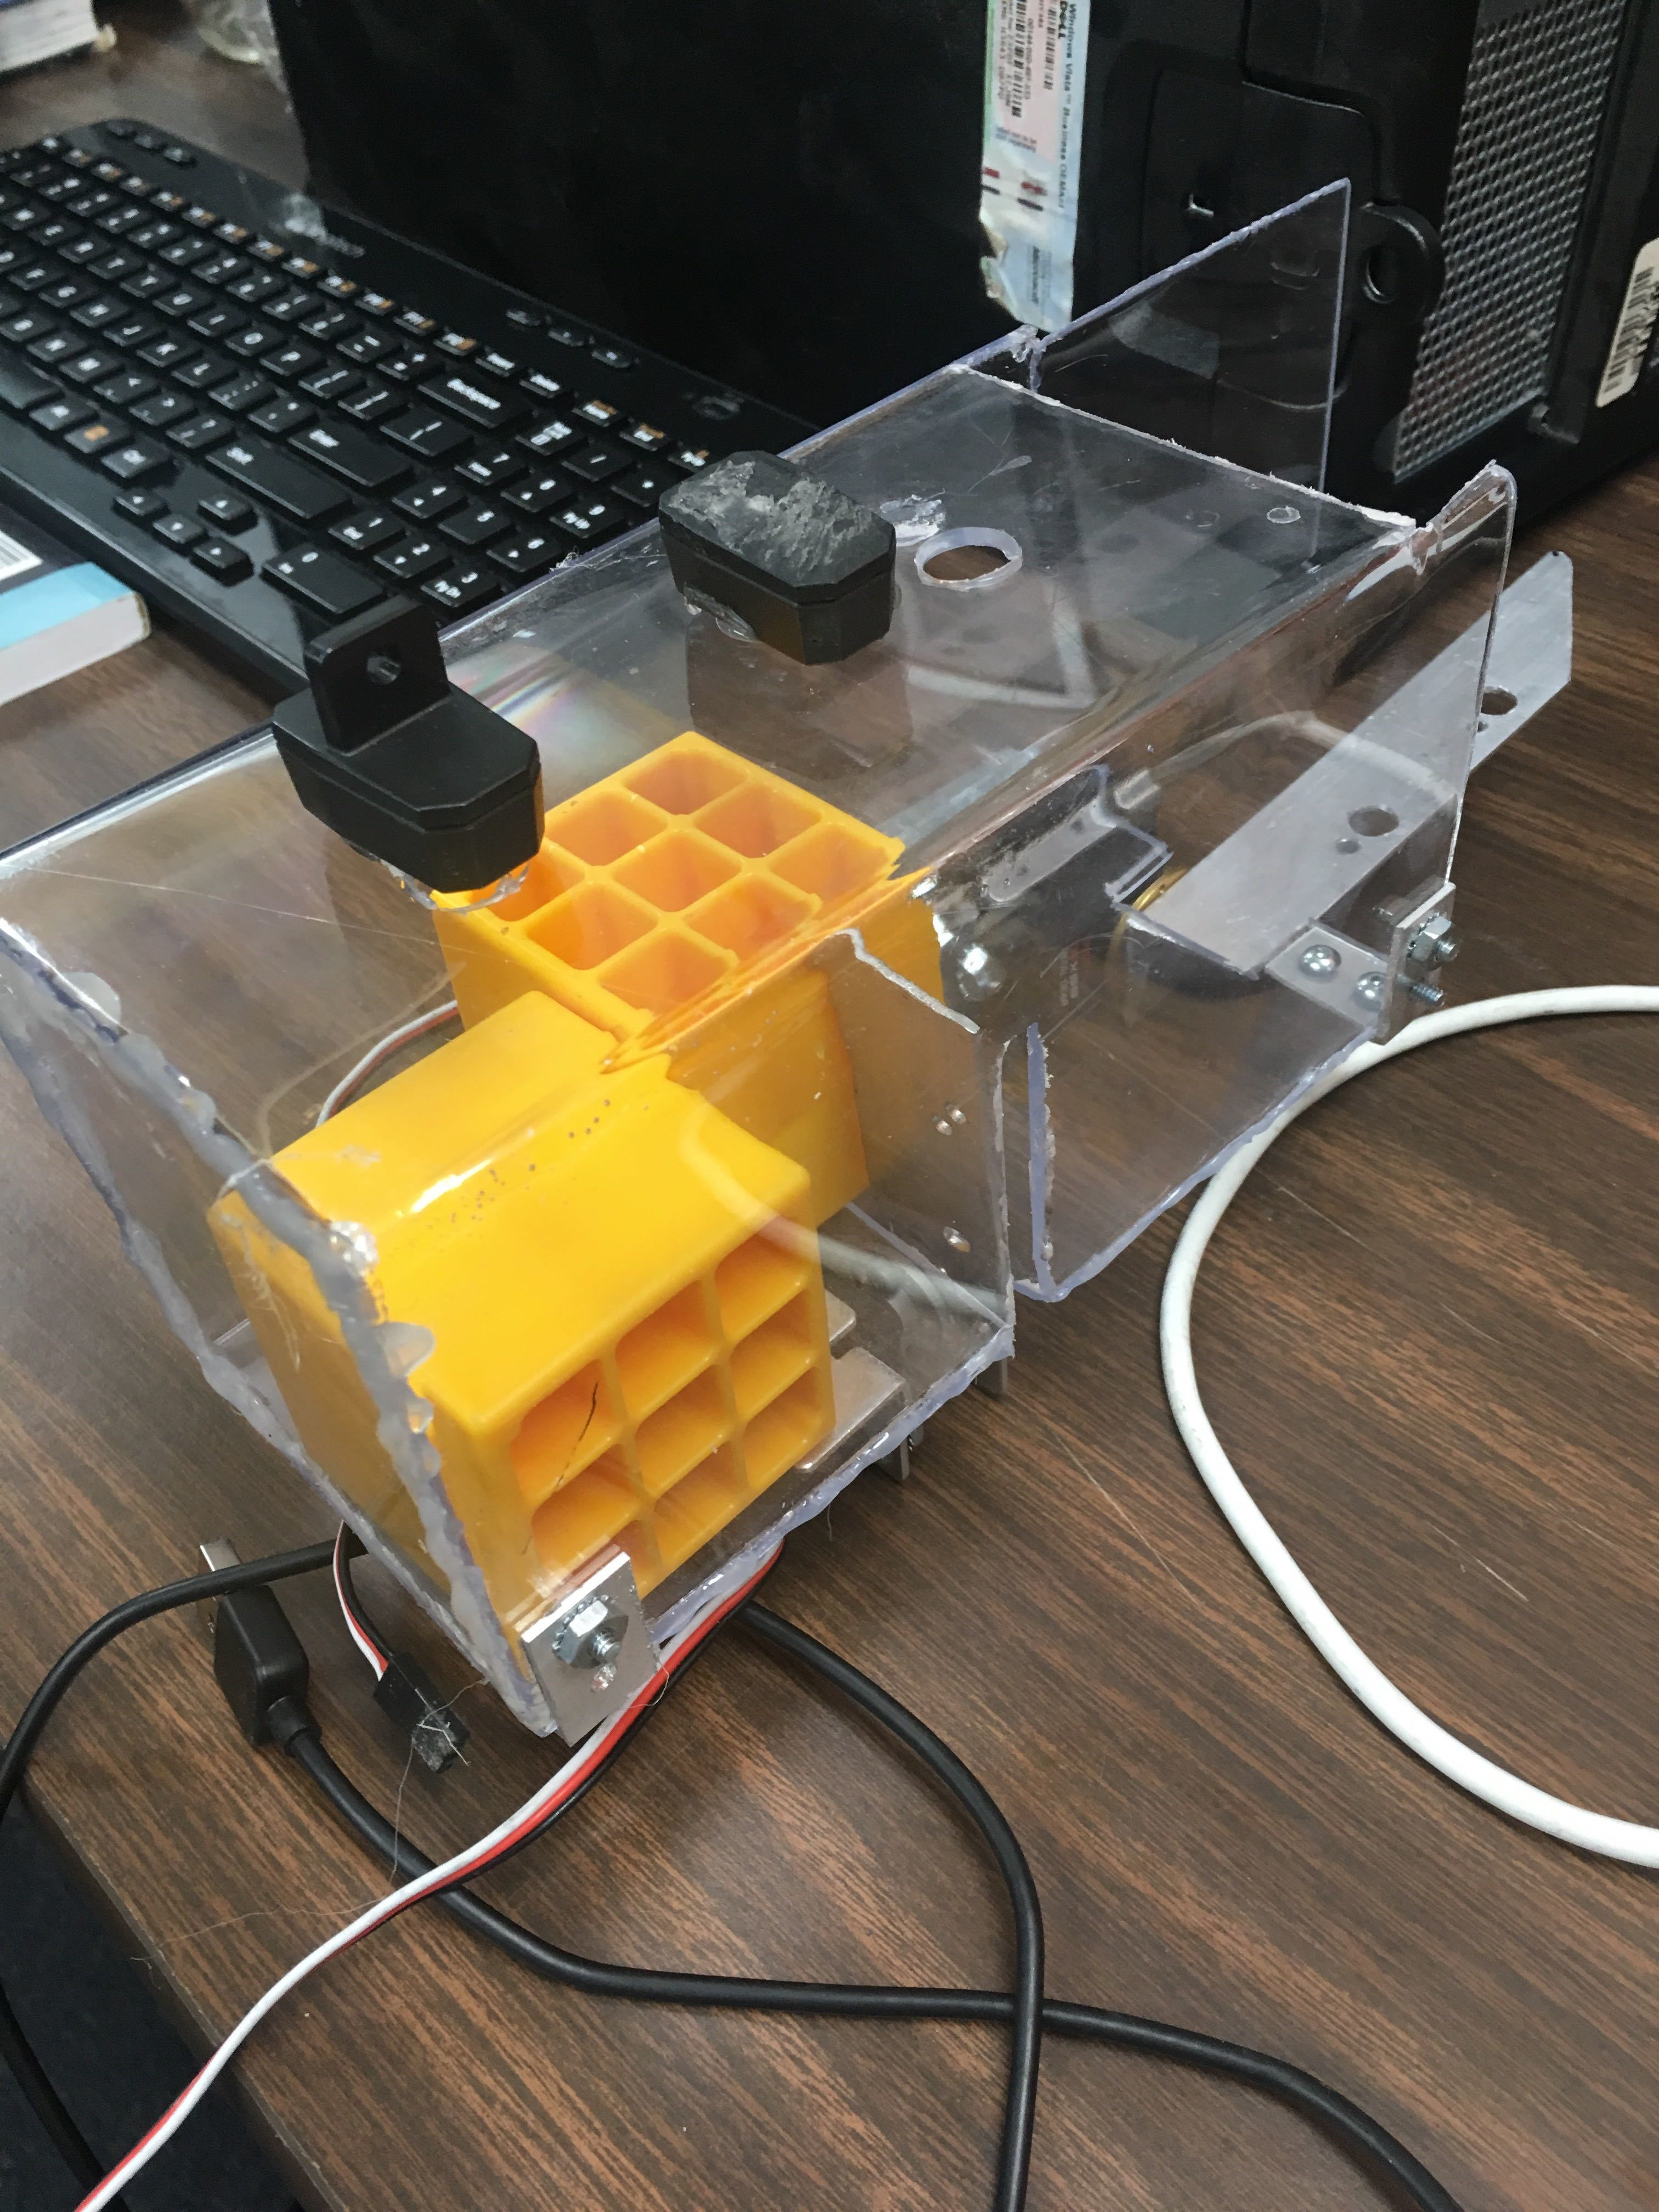
\includegraphics[width=.6 \textwidth]{15_12-10/images/Diverter.jpg}
    \caption{Diverter Design}
    \label{fig:diverter}
\end{figure}

\subsection{Testing X-Rail Slides}
%! Testing and assembling the X-Rail slides.
Now that the X-rail had arrived from order, the team saw fit to construct a set of X-rail for testing. Jon, Ben, and Shawn took on this task. Given that the X-rail was as yet unproven, it was important to run it through its paces to ensure it was a good option. While on paper the X-rail was perhaps the best option for the horizontal linear motion the team was looking for, in practice things could be different. After Jon, Ben, and Shawn completed the X-rail kit, Jon began testing the X-rail slide. He tested that the surgical tubing was taught enough to pull blocks and balls back to the intake, he tested how and where it would be mounted, he tested the rigging, and he tested where the servo for the rake would mount. After testing all these qualities, Jon determined that the X-rail would be a good replacement for the Rev Linear slides. While the X-rail would function in almost the same way as the Rev linear slides; A couple things would have to be changed. The rake servo would have to be mounted lower, and the rake would have to rotate from side to side rather than up and down. Being that the X-rail is larger than the Rev slides, the rake servo would need to be mounted lower so the rake could be as close to the ground as possible. Even with the servo being mounted lower, it was still high enough off the ground that the rake would have to deploy in a different way. The team decided that having the rake swing down from the X-rail would not only be a more efficient use of space, reduce wobble and strain, but would also more easily allow the use of X-rail. This would require the design of a new rake which set to work on. 




\end{document}